\documentclass[a4paper,10pt,openright]{report}
\setlength{\parindent}{0pt} % set noindent for entire file

\usepackage[utf8]{inputenc}
\usepackage[a4paper, top=2cm, left=1cm, right=1.5cm]{geometry}
\usepackage{xcolor,graphicx}
\usepackage{amsmath}
\usepackage{setspace}
\usepackage{sectsty}
\usepackage{etoolbox}
\usepackage{enumitem}
\usepackage{listings}
\usepackage{times}

\graphicspath{ {/home/saran/Analytics/May_04/} }

\lstdefinestyle{mystyle}{
	backgroundcolor=\color{white},
	basicstyle=\ttfamily\footnotesize,
	breakatwhitespace=false,
	breaklines=true,
	captionpos=b,
	keepspaces=true,
	showspaces=false,
	showstringspaces=false,
	showtabs=false,
	tabsize=4
}

\lstset{style=mystyle}

\begin{document}
\singlespacing
\pagestyle{plain}

\begin{center}
\textbf{Assignment Poisson Distribution} \\
Date: 04/05/2020 \hspace{2mm} Name: D.Saravanan
\end{center}

\vspace{10px}

\begin{enumerate}

\item[1.] Find the probability that at most $5$ defective fuses will be found in a box of 
$200$ fuses if experience shows that $2$ percent of such fuses are defective. \\

Poisson Distribution Formula:
\begin{equation*}
P(X = k) = \frac{\lambda^{k} e^{-\lambda}}{k!}
\end{equation*}

where, \\
$k = 0, 1, 2, 3,..., \infty$\\
$\lambda$ = mean number of occurrences in the interval \\
$e$ = Euler's constant $\approx 2.71828$ \\


$N = 200$ and $p = 1/50$ \\
Expectation value of $k$, $E[k] = \lambda = 200 \times 1/50 = 4$



\begin{equation*}
P(X \leq 5)  = \sum_{k=0}^{5} \frac{\lambda^{k} e^{-\lambda}}{k!}
		     = \sum_{k=0}^{5} \frac{4^{k} e^{-4}}{k!}
			 = 0.7851
\end{equation*}

Program:
\lstinputlisting[language=Python]{pdistribution.py}

Output:
\lstinputlisting{outputp2.txt}

\vspace{1cm}

\item[2.] The number of accidents in a year attributed to taxi drivers in a city follows a
Poisson distribution with mean equal to $3$. Out of $1000$ taxi drivers, find approximetly
the number of drivers with \\

\begin{enumerate}

\item[a)] No accidents in a year 
\begin{equation*}
P(X = 0) = \frac{3^{0} e^{-3}}{0!} = 0.0498
\end{equation*}

\item[b)] More than $3$ accidents in a year 
\begin{equation*}
\begin{split}
		P(X > 3) & = 1 - P(X \leq 3) \\ 
		& = 1 - (P(X = 0) + P(X = 1) + P(X = 2) + P(X = 3)) \\
		& = 1 - \left( \frac{3^{0} e^{-3}}{0!} + \frac{3^{1} e^{-3}}{1!} + \frac{3^{2} e^{-3}}{2!} + \frac{3^{3} e^{-3}}{3!} \right) \\
		& = 1 - (0.0498 + 0.1494 + 0.2240 + 0.2240) \\
		& = 0.3528
\end{split}
\end{equation*}

\end{enumerate}

\pagebreak

Program:
\lstinputlisting[language=Python]{pdist.py}

Output:
\lstinputlisting{outputp1.txt}

\pagebreak

Program: Scipy package
\lstinputlisting[language=Python]{taxi.py}

Output:
\lstinputlisting{outputp3.txt}

\item[3.] From the records of $10$ Indian Army corps kept over $20$ years the following data
were obtained showing the number of deaths caused by the horse. Calculate the theoretical
Poisson frequencies. \\
\begin{tabular}{|l|r|r|r|r|r|}
\hline
No. of Deaths: & 0 & 1 & 2 & 3 & 4 \\
\hline
Frequency : & 109 & 65 & 22 & 3 & 1 \\
\hline
\end{tabular} \\

$N = 109 + 65 + 22 + 3 + 1 = 200$ \\ \\
$\sum_{}^{} k \cdot F = 0 \cdot 109 + 1 \cdot 65 + 2 \cdot 22 + 3 \cdot 3 + 4 \cdot 1 = 122$ \\ \\
Mean, $\lambda = (\sum_{}^{} k \cdot F)/N = 122/200 = 0.61$ \\

Calculation of Probability:
\begin{equation*}
		\begin{split}
				P(X = 0) & = \frac{(0.61)^{0} e^{-0.61}}{0!} = 0.5433 \\
				P(X = 1) & = \frac{(0.61)^{1} e^{-0.61}}{1!} = 0.3314 \\
				P(X = 2) & = \frac{(0.61)^{2} e^{-0.61}}{2!} = 0.1011 \\
				P(X = 3) & = \frac{(0.61)^{3} e^{-0.61}}{3!} = 0.0206 \\
				P(X = 4) & = \frac{(0.61)^{4} e^{-0.61}}{4!} = 0.0031
		\end{split}
\end{equation*}

\begin{tabular}{|l|r|r|r|r|r|}
\hline
No. of Deaths : & 0 & 1 & 2 & 3 & 4 \\
\hline
Frequency : & 109 & 65 & 22 & 3 & 1 \\
\hline
Calculated Frequency, $N \cdot P(k)$ : & 108.7 & 66.3 & 20.2 & 4.1 & 0.6 \\
\hline
\end{tabular}

Program:
\lstinputlisting[language=Python]{pfrequency.py}

Output:
\lstinputlisting{outputp4.txt}

Program: Scipy package
\lstinputlisting[language=Python]{calculated.py}

\begin{figure}[ht!]
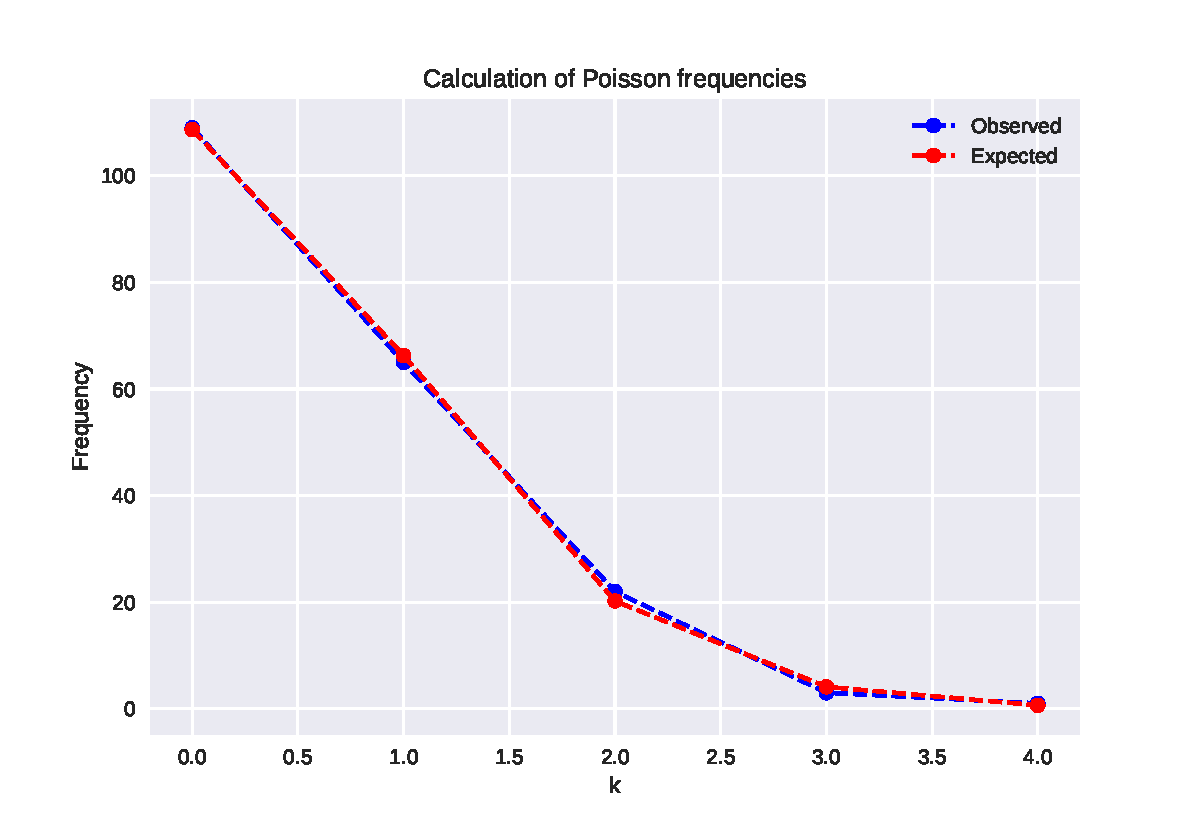
\includegraphics[width=18cm,height=9cm,keepaspectratio]{frequency.pdf}
\centering
\end{figure}

\end{enumerate}
\end{document}
